\documentclass[12pt]{article}
\usepackage[margin=1in]{geometry} % Set margins to 1 inch
\usepackage{amsmath} % Advanced math typesetting
\usepackage{amsfonts} % Additional math fonts
\usepackage{amssymb} % Extended symbol collection
\usepackage{graphicx} % For including images
\usepackage{enumitem} % Customize list environments
\usepackage[most]{tcolorbox} % Load the tcolorbox package with additional libraries

\setlength{\parindent}{0pt} % Removes all indentation from paragraphs

\newtcolorbox{mybluebox}[1][]{
  colback=teal!15!white,
  colframe=teal!50!black,
  title=#1
}

\begin{document}

\title{Math 164 HW 2}
\author{Shilpa Bojjireddy}
\maketitle


\begin{mybluebox}
    \textbf{1.} Let $f(x) = x^2 + 4\cos{x}, x \in \mathbb{R}$. We wish to find the minimizer $x^*$ of $f$ over the interval $[1,2]$. 
    (Calculator users: Note that in $\cos x$, the argument $x$ is in radians.)
    
    \begin{itemize}
        \item[(a)] Plot $f(x)$ versus $x$ over the interval $[1,2]$.
        
        \item[(b)] Use the golden section method to locate $x^*$ to within an uncertainty of $0.2$. Display all intermediate steps using a table:
        
        \begin{center}
        \begin{tabular}{|c|c|c|c|c|c|}
        \hline
        Iteration $k$ & $a_k$ & $b_k$ & $f(a_k)$ & $f(b_k)$ & New uncertainty interval \\
        \hline
        1 & ? & ? & ? & ? & [?, ?] \\
        2 & ? & ? & ? & ? & [?, ?] \\
        \vdots & \vdots & \vdots & \vdots & \vdots & \vdots \\
        \hline
        \end{tabular}
        \end{center}
        
        \item[(c)] Repeat part (b) using the bisection method, with $\epsilon = 0.05$. Display all intermediate steps using a table.
        
        \item[(d)] Apply Newton's method, using the same number of iterations as in part (b), with $x^{(0)} = 1$.
    \end{itemize}
\end{mybluebox} 
\textbf{Solution: } \\
\begin{itemize}
    \item[(a)] 
        \begin{minipage}{0.6\textwidth}
        \end{minipage}
        \begin{minipage}{0.4\textwidth}
            \centering
            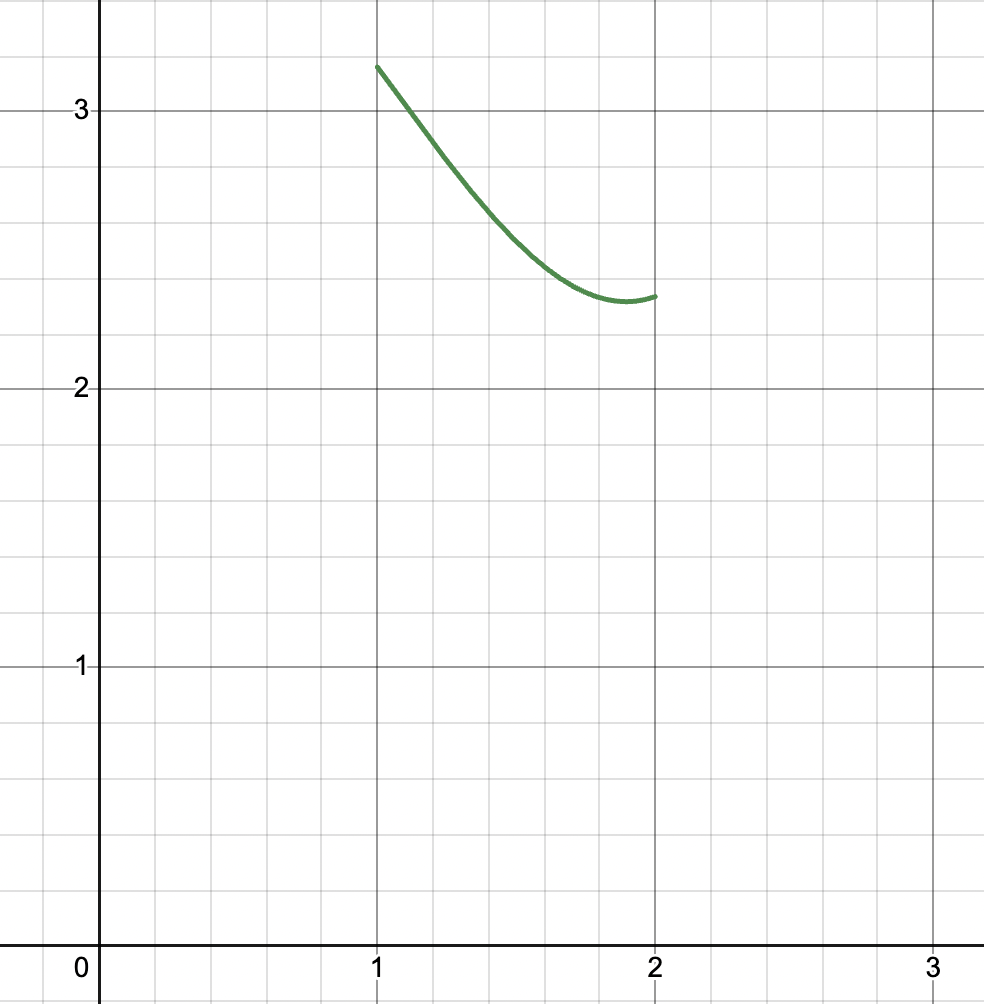
\includegraphics[width=\textwidth]{1a.png} 
        \end{minipage}
    \item[(b)] 
    \begin{tabular}{|c|c|c|c|c|c|}
        \hline
        Iteration $k$ & $a_k$ & $b_k$ & $f(a_k)$ & $f(b_k)$ & New uncertainty interval \\
        \hline
        1 & 1.618 & 1.382 & 2.429 & 2.661 & [1.382, 2] \\
        2 & 1.764 & 1.618 & 2.343 & 2.430 & [1.618, 2] \\
        3 & 1.854 & 1.764 & 2.320 & 2.434 & [1.764, 2] \\
        4 & 1.910 & 1.854 & 2.317 & 2.320 & [1.854, 2] \\
        \hline
    \end{tabular} \\ \\ 
    We found x* in 4 iterations, it is located in the interval [1.854, 2] 
    \item[(c)]
    $f(x) = x^{2} + 4cos(x) \implies f'(x) = 2x - 4sin(x)$  \\

    \begin{tabular}{|c|c|c|c|c|c|}
        \hline
        Iteration $k$ & $a_k$ & $b_k$ & $m$ & $f'(m)$ & New uncertainty interval \\
        \hline
        1 & 1 & 2 & 1.5 & -0.989 & [1.5, 2] \\
        2 & 1.5 & 2 & 1.75 & -0.436 & [1.75, 2] \\
        3 & 1.75 & 2 & 1.875 & -0.066 & [1.875, 2] \\
        4 & 1.875 & 2 & 1.938 & 0.140 & [1.875, 1.938] \\
        5 & 1.875 & 1.938 & 1.906 & 0.036 & [1.875, 1.906] \\
        \hline
    \end{tabular}

    \item[(d)] 
    Newton's Method : $x_{n+1} = x_n - \frac{f'(x_{n})}{f''(x_{n})}$\\
    $f''(x) = 2 - 4cos(x)$
    \\ \\
    \begin{tabular}{|c|c|c|c|c|c|}
        \hline
        Iteration $k$ & $x_n$ & $x_{n+1}$  \\
        \hline
        1 & 1 & -7.473 \\
        2 & -7.473 & 14.479 \\
        3 & 14.479 & 6.935 \\
        4 & 6.935 & 16.636 \\
        \hline
    \end{tabular}

\end{itemize}

\bigbreak

\begin{mybluebox}
    \textbf{2.} Suppose that \( \rho_1, \dots, \rho_N \) are the values used in the Fibonacci search method. Show that for each \( k = 1, \dots, N \), \( 0 \leq \rho_k \leq \frac{1}{2} \), and for each \( k = 1, \dots, N - 1 \),
    \[
    \rho_{k+1} = 1 - \frac{\rho_k}{1 - \rho_k}.
    \]
    \end{mybluebox}
    
    Recall that \( \rho_k = 1 - \frac{F_{N-k+1}}{F_{N-k+2}} \). Since \( F_N \) represents a Fibonacci number, which is always positive by the definition of the Fibonacci sequence, we know that \( \frac{F_{N-k+1}}{F_{N-k+2}} > 0 \) for all \( N \).
    
    Moreover, since by the definition of the Fibonacci sequence, \( F_{N-k+1} + F_{N-k} = F_{N-k+2} \), we also know that \( F_{N-k+2} > F_{N-k+1} \), and thus \( \frac{F_{N-k+1}}{F_{N-k+2}} < 1 \), which implies \( 0 < \rho_k \).
    
    To show that \( \rho_k < \frac{1}{2} \), we use the fact that the ratio of consecutive Fibonacci numbers converges to the golden ratio \( \phi \approx 1.618 \):
    \[
    \lim_{n \to \infty} \frac{F_{n+1}}{F_n} = \phi.
    \]
    Thus, for large \( N \), we have:
    \[
    \rho_k = 1 - \frac{F_{N-k+1}}{F_{N-k+2}} \approx 1 - \frac{1}{\phi}.
    \]
    Since \( \phi \approx 1.618 \), we have:
    \[
    \frac{1}{\phi} \approx 0.618,
    \]
    and therefore:
    \[
    \rho_k \approx 1 - 0.618 = 0.382 < \frac{1}{2}.
    \]
    Thus, we conclude that \( 0 < \rho_k < \frac{1}{2} \) for all \( k \).
    
\bigbreak
Now, We want to show that $$ \rho_{k+1} = 1 - \frac{\rho_k}{1 - \rho_k} $$

We know that for the Fibonacci search method, $$\rho_{k} = 1- \frac{F_{N-k-1}}{F_{N-k+2}} \implies 1-\rho_{k} = \frac{F_{N-k+1}}{F_{N-k+2}} $$
and $$\rho_{k+1} = 1- \frac{F_{N-k}}{F_{N-k+1}}    (*) $$ 
Now, to prove the recurrence relation, it will suffice to show that 
$$ 1 - \frac{\rho_k}{1 - \rho_k} = 1- \frac{F_{N-k}}{F_{N-k+1}} \implies \frac{\rho_k}{1 - \rho_k} = \frac{F_{N-k}}{F_{N-k+1}}$$

\begin{align}
    \frac{\rho_k}{1 - \rho_k} &= \frac{F_{N-k}}{F_{N-k+1}} \\
    (\rho_k)(F_{N-k+1}) &= (1 - \rho_k)(F_{N-k})  \\
    (1- \frac{F_{N-k-1}}{F_{N-k+2}})(F_{N-k+1}) &= (\frac{F_{N-k+1}}{F_{N-k+2}})(F_{N-k}) \\
    F_{N-k+2} - F_{N-k-1}*F_{N-k+1} &= F_{N-k+1}*F_{N-k}\\
    F_{N-k}*F_{N-k+1} &= F_{N-k+1}*F_{N-k}
\end{align}
We go from (4) to (5) because by the Fibonacci Sequence definition, $F_{N-k+1} + F_{N-k} = F_{N-k+2}$. \\
Since we know $(*)$, we have shown for each $k = 1, \dots, N - 1$, $\rho_{k+1} = 1 - \frac{\rho_k}{1 - \rho_k}$

\bigbreak

\begin{mybluebox}
\textbf{3.} Suppose that we have an efficient way of calculating exponentials. Based on this, use Newton’s
method to devise a method to approximate $log(2)$ [where ”log” is the natural logarithm function].
Use an initial point of $x^{(0)} = 1$, and perform two iterations.
\end{mybluebox}
Newton's Method : $x_{n+1} = x_n - \frac{f'(x_{n})}{f''(x_{n})}$
To use Newton's Method to approximate $ln(2)$, we will rewrite this as a "finding the minimum" problem, where our minimum, $x^*$ is at $ln(2)$ \\
Let $f(x) = (e^{x} - 2)^2$, the minimum is at $f(x) = 0 \implies x^*=ln(2)$ \\
To approximate the minimum, $x^*$, let's apply Newton's method on $f(x)$ \bigbreak
\begin{tabular}{|c|c|c|c|c|c|}
    \hline
    Iteration $k$ & $x_n$ & $x_{n+1}$  \\
    \hline
    1 & 1 & 0.838 \\
    2 & 0.838 & 0.752\\
    \hline
\end{tabular}\\ \\
After 2 iterations of Newton's method, we conclude that $log(2) \approx 0.751$
\bigbreak
\begin{mybluebox}
    \textbf{4.} Consider the problem of finding the zero of $g(x) = (e^x - 1)/(e^x + 1)$, $x \in \mathbb{R}$, where $e^x$ is the exponential of $x$. (Note that $0$ is the unique zero of $g$.)
    \begin{itemize}
        \item[(a)] Write down the algorithm for Newton’s method of tangents applied to this problem. Simplify using the identity $\sinh{x} = (e^x - e^{-x})/(2)$.
        
        \item[(b)]Find an initial condition $x^{(0)}$ such that the algorithm cycles [i.e. $x^{(0)} = x^{(2)} = x^{(4)} = \cdots$]. You need not explicitly calculate the initial condition; it suffices to provide an equation that the initial condition must satisfy. \textit{Hint:} Draw a graph of $g$.
        
        \item[(c)] For what values of the initial condition does the algorithm converge?
    \end{itemize}
\end{mybluebox}
(a.) Newton's method for tangents is $x^{k+1} = x^k - \frac{g(x^k)}{g'(x^k)}$
\begin{align}
    g(x) &= \frac{(e^x - 1)}{(e^x + 1)} \\
    g'(x) &= \frac{2e^x}{(e^x+1)^2}\\
    \frac{g(x)}{g'(x)} &= \frac{(e^x-1)(e^x+1)}{2e^x} \\
     &= \frac{1}{2}(e^x-e^{-x}) = sinh(x)\\
    x^{k+1} &= x^k -  sinh(x)
\end{align}

(b.) 
\begin {align}
x^0 &= x^2\\
x^1 &= x^0 - sinh(x^0) \\
x^2 &= x^1 - sinh(x^1) \\
x^0 &= (x^0 - sinh(x^0)) - sinh((x^0 - sinh(x^0))) \\
0 &= (- sinh(x^0)) - sinh((x^0 - sinh(x^0)))
\end{align}

The initial condition, $x^0$, must satisfy equation (15) \\

(c.) For the algorithm to converge, the initial condition must not cycle.  \\
$ \forall x>0, x < sinh(x)$ and $\forall x<0, x > sinh(x) $ \\
By Newton's method, we have $ x^{k+1} = x^k - sinh(x) $ \\
So, for $x>0$, $|x-sinh(x)| < x \implies -x < x-sinh(x) \implies sinh(x) < 2x $\\
And conversely, for $x<0 \implies sinh(x) > 2x$ \\
The algorithm is likely to converge in the interval between the values $ \pm (\frac{sinh(x)}{x} = 2)$, this is approximately the interval $[-2.177, 2.177]$
\bigbreak

\begin{mybluebox}
    \textbf{5.} Consider using a gradient algorithm to minimize the function
    \[
    f(x) = \frac{1}{2} x^{\top} \begin{bmatrix} 2 & 1 \\ 1 & 2 \end{bmatrix} x
    \]
    with the initial guess $x^{(0)} = \begin{bmatrix} 0.8 \\ -0.25 \end{bmatrix}^{\top}$.

    \begin{itemize}
        \item[(a)] To initialize the line search, apply the bracketing procedure in Figure 7.11 (in the book) along the line starting at $x^{(0)}$ in the direction of the negative gradient. Use $\epsilon = 0.075$.

        \item[(b)] Apply the golden section, Fibonacci or bisection method to reduce the width of the uncertainty region to 0.01. Organize the results of your computation in a table format similar to that of Exercise 2.
    \end{itemize}
\end{mybluebox}

(a) Let's first calculate the negative gradient. Recall that a quadratic function in the form $f(x)=x^{\top}Qx$, has a gradient of the form $\nabla f(x) = 2Qx$.
\begin{align}
    \nabla f(x^{(0)}) &= 2Qx^{(0)}  \\
    \nabla f(x^{(0)}) &= 2 \begin{bmatrix} 1 & 0.5 \\ 0.5 & 1 \end{bmatrix} \begin{bmatrix} 0.8 \\ -0.25 \end{bmatrix} = \begin{bmatrix} 1.35 \\ 0.3 \end{bmatrix} \\
    x_{k+1} &= x_k - 2^k\epsilon  \nabla f(x^{(0)}) \\
    x_{k+1} &= \begin{bmatrix} 0.8 \\ -0.25 \end{bmatrix} - 0.075 \begin{bmatrix} 1.35 \\ 0.3 \end{bmatrix}
\end{align}
Using Python, I computed a few iterations of the bracketing procedure to calculate the desired bracket.\\ 
\\
\begin{minipage}{1.2\textwidth}
\end{minipage}
\begin{minipage}{0.8\textwidth}
    \centering
    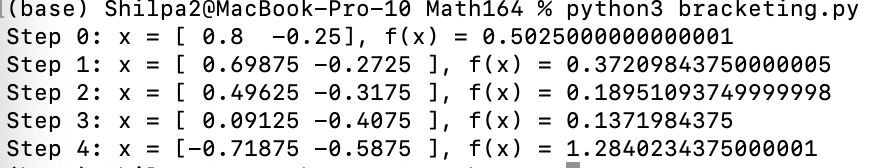
\includegraphics[width=\textwidth]{bracketing.png} 
\end{minipage} 
\\ \\ From these results, we can observe that the desired bracket is between iterations 2 through 4, where
$ a = x_2 = [0.496, -0.318], c  = x_3 = [0.091, -0.408], b = x_4 = [-0.719, -0.588]$.
\\
(b) Let's use the Golden Section method. \\ \\
Using Python, I obtained these results:
\\
\noindent
\hspace*{-2.4cm}
\begin{minipage}{1.3\textwidth}
    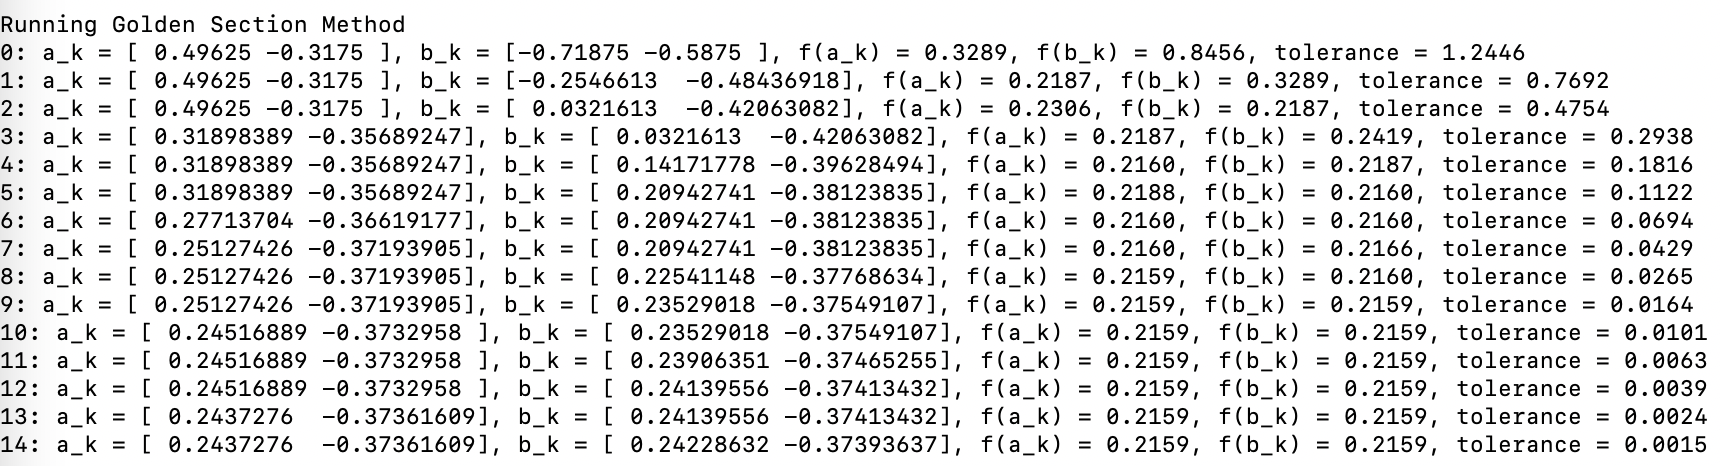
\includegraphics[width=\textwidth]{golden_section.png} 
\end{minipage}
\\

\end{document}
